
\begin{figure}[!tpb]
  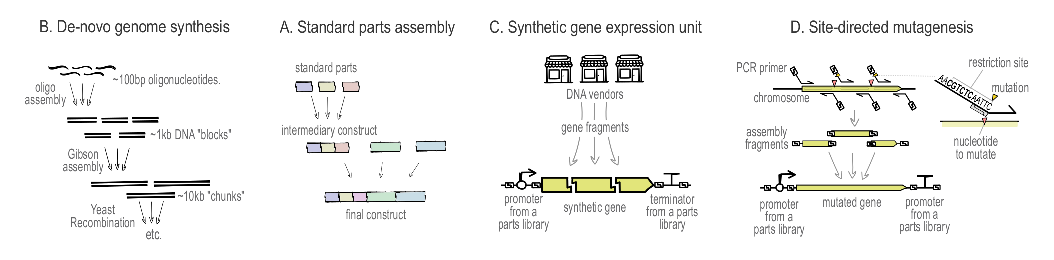
\includegraphics[width=\textwidth]{figures/figure_1_dna_projects.eps}
  \caption{Illustration of different categories of DNA construction projects. The schemas focus on the assembled parts and do not show the plasmid backbones necessary for assembly selection and amplification. \textbf{(A)} First steps of the hierarchical assembly of an artificial chromosome in the Sc2.0 project.
\textbf{(B)} 2-step assembly of standard genetic parts. The second step can use a mix of intermediary constructs and standard genetic parts.
\textbf{(C)} Golden Gate Assembly of a gene expression unit using standard promoter and terminator parts from a library, and a long synthetic gene bought in three fragments from commercial vendors, resulting in a five-part assembly.
\textbf{D} Assembly of a gene expression unit using standard promoter and terminator parts, as in Panel C, but where the gene obtained from the chromosome of an organism via PCR. Red triangles on the chromosome indicate the position of BsmBI sites which preclude Golden Gate assembly, and are mutated away in the final sequence.}
  \label{dna_projects}
\end{figure}


\begin{figure}[!tpb]
  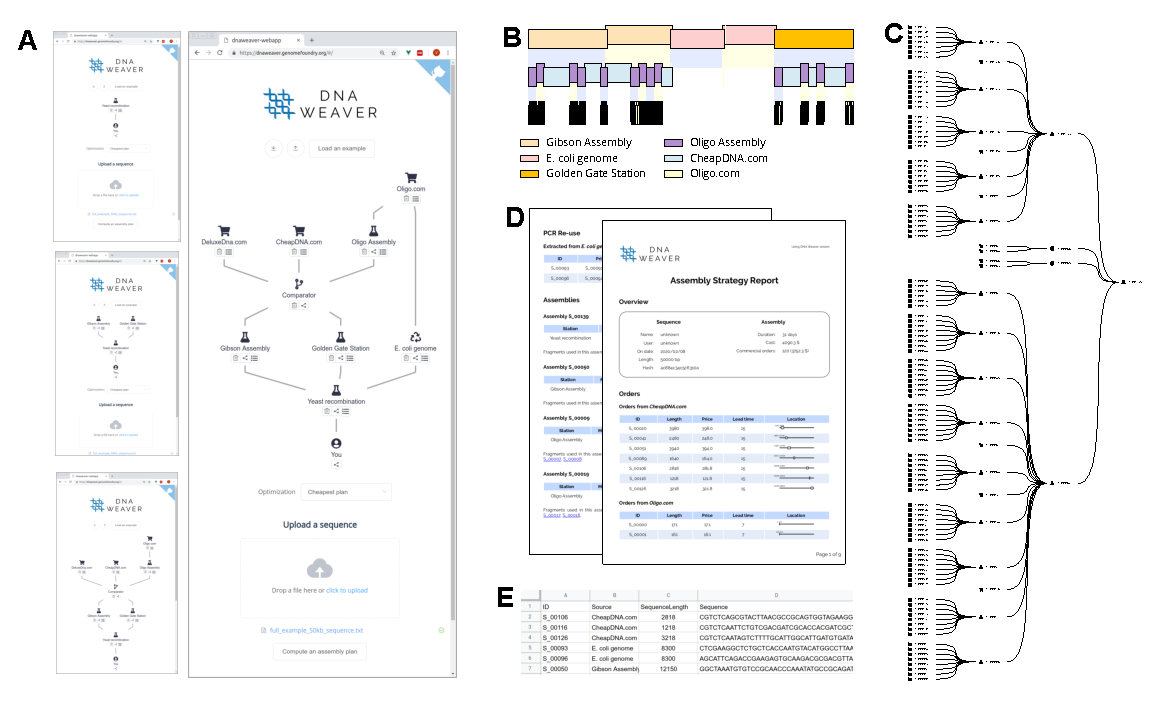
\includegraphics[width=\textwidth]{figures/figure_2_app_screenshots.eps}
  \caption{The DNA Weaver web application and its output. The scenario described in this figure can be loaded and experimented with via the "Load an example" button of the web application.
\textbf{(A)} DNA supply network defined via the web interface. Miniatures on the left show the chronological order of the network's construction. Small icons under a station lead to menus to select parameters and suppliers.
\textbf{(B)} Schema of the multi-step construction plan (from bottom to top) of a 50kb sequence, devised by the web application with respect to the supply network in Panel A, in under 10 seconds. Each rectangle represents a DNA fragment whose color indicates the provenance. The top line shows the fragments of the final assembly: the plan takes advantage of a large homology of the sequence with \textit{E. coli} to obtain the central part via PCR. The second line shows the origin of the blocks used in Gibson Assembly or Golden Gate assembly. In this plan, the fragments come either from CheapDNA or the assembly of oligonucleotides (represented on the third line). This schema is appears as a PDF file in the multi-file report generated by DNA Weaver.
\textbf{(C)} Summary PDF report indicating the different assembly steps and listing all assembly fragments ordered or built.
\textbf{D} Spreadsheet listing the sequence of every fragment or primer to order, and every assembled fragment.
\textbf{E} Map of the assembly plan providing an alternative view to the Panel B schema, with the identifiers of the different fragments and primers involved in the assembly.}
  \label{app_screenshots}
\end{figure}



\begin{figure}[!tpb]
  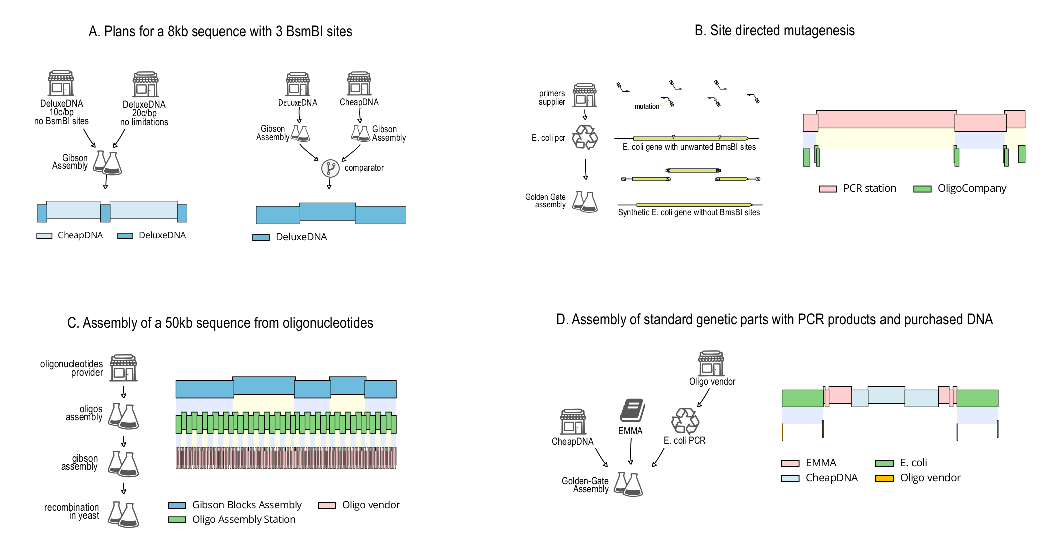
\includegraphics[width=\textwidth]{figures/figure_3_example_supply_networks.eps}
  \caption{
Examples of DNA Weaver supply networks for different DNA Construction problems. The assembly plan summary plots in each panel can be generated using the examples provided in the DNA Weaver Github repository. Each rectangle represents an assembly fragment or primer, and colors indicate each fragment's origin (see the caption of Figure 2B for details).
\textbf{(A)} Multi-vendor problem. A 10kb DNA sequence containing 3 BsmBI restriction sites will be assembled via Gibson assembly using fragments comming from one of two vendors: CheapDNA charges 10c per basepair but won't synthesize fragments containing a BsmBI site. DeluxeDNA can produce any fragment for 20c/bp. Both stations only sell fragments under 4kb. In the left network, each fragment can be ordered from a different vendor, resulting in a plan using CheapDNA as much as possible, and DeluxeDNA only in regions harboring a BsmBI site. The right-hand network compares two assembly workflows where all DNA fragments come from a single source. As a result, the assembly plan suggested catters to the cheapest provider able to provide all fragments at once.
\textbf{B} Site directed mutagenesis, as presented in Figure 1C. This problem can be modelled as a linear supply network comprising a commercial primers vendor, an \textit{E. coli} PCR station, and a Golden Gate Assembly station. The sequence to assemble, a synthetic \textit{E. coli} gene edited to remove BsmBI sites, will be created by ordering primers from the vendor, using them in the PCR station to amplify the chromosome fragments to be assembled.
\text{C} Hierarichical assembly of an arbitrary sequence from oligonucleotides. This example mimics the protocol of Figure 1A with a linear supply network chaining different assembly stations which feed each other with increasingly large DNA fragments.
\text{D} Supply network for the assembly of a gene expression unit from various sources. The sequence to build contained a coding sequence that must be ordered commercially, flanked by 6 standard parts from the EMMA Assembly standard, and 2 homology harms for integration in \textit{E. coli}. The assembly plan correctly detected that the reusable EMMA parts and homologies.}
  \label{app_screenshots}
\end{figure}


\begin{figure}[!tpb]
  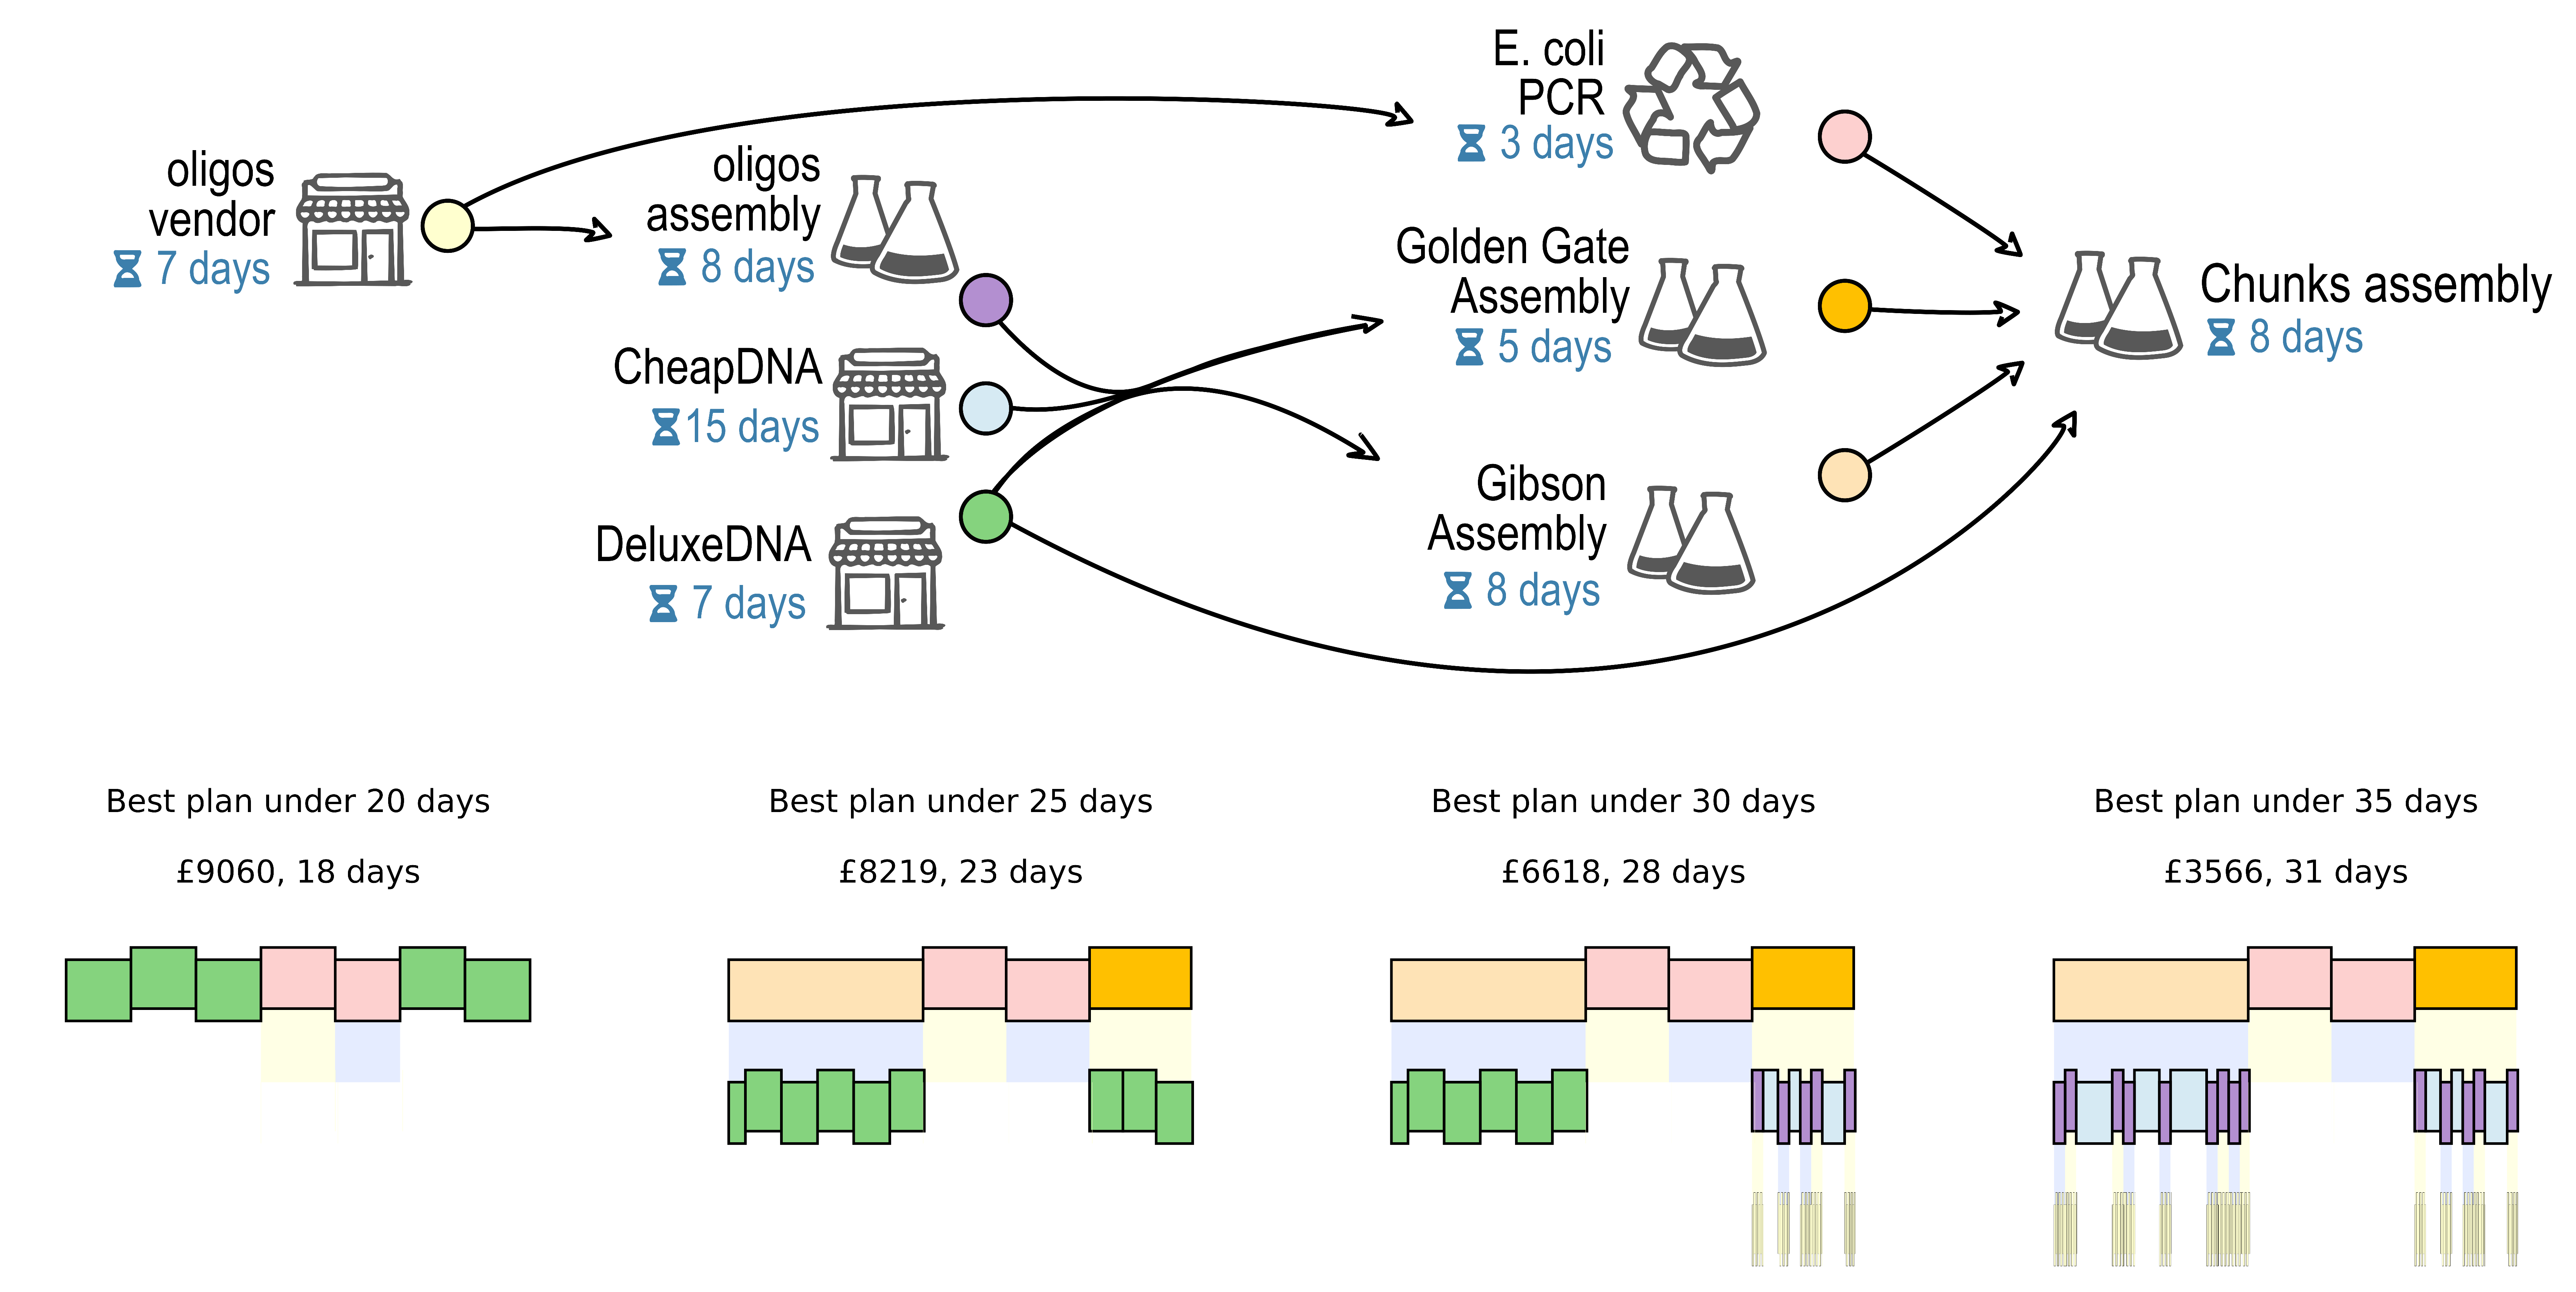
\includegraphics[width=\textwidth]{figures/figure_4_time_limit.eps}
  \caption{Effect of lead time constraints on the assembly plan returned by DNA Weaver. The supply network is a variant of the network described in Figure 1, where the typical lead time of each station, in days, is specified. The assembly plots below show four plans computed for the sequence of Figure 1, but for increasing large maximal lead times used as parameters.} 
  \label{lead_time}
\end{figure}


\begin{figure}[!tpb]
  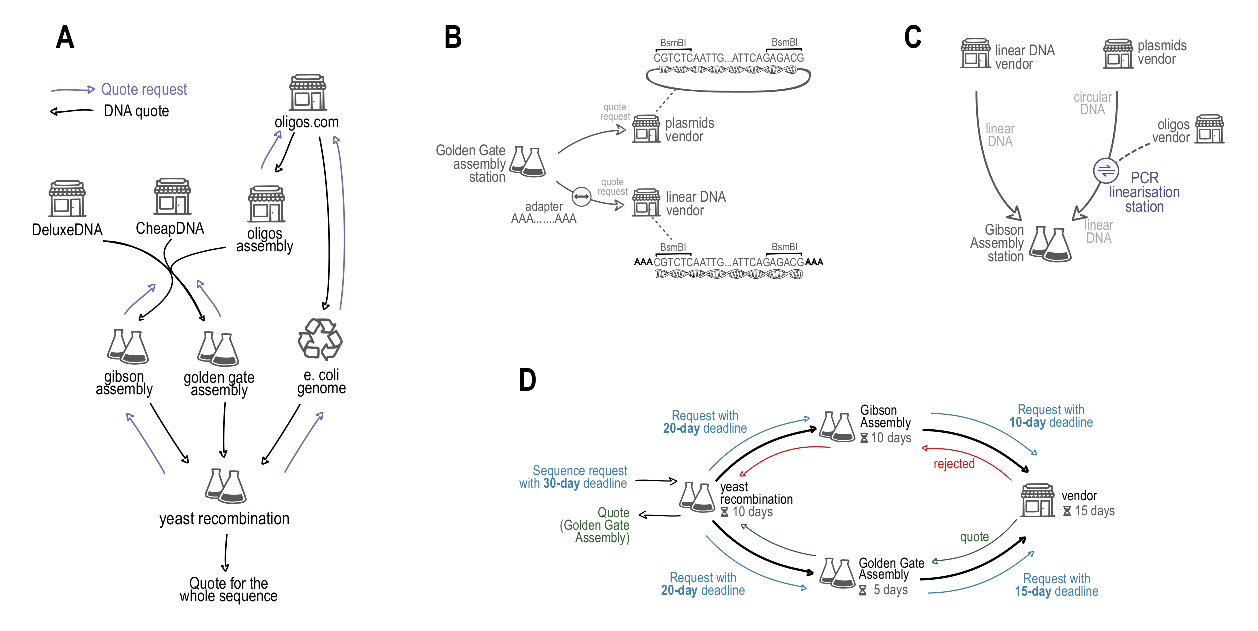
\includegraphics[width=\textwidth]{figures/figure_5_supply_networks_function.eps}
  \caption{Exchanges between the stations of a supply network.
  \textbf{(A)} Direction of requests and sequence quotes in the supply network of Figure 2A.
  \textbf{(B)} Supply network where a same sequence, flanked by cloning restriction sites, can be requested to two different suppliers producing respectively linear and circular DNA. A sequence extension station is intercaled before the linear DNA vendor to add a few basepairs to the sequence flanks and avoid having the restriction sites at the end of the sequence.
  \textbf{C} Two vendors, offering respectively linear and circular DNA, supply fragments for a Gibson Assembly. A PCR linearization station and a primers supplier are added before the circular DNA vendor, to take into account the linearization of fragments required by Gibson Assembly.
  \textbf{D} Example of requests and responses between the elements of a network in presence of a maximal lead time constraint. Here it is assumed that the researcher modeled Gibson Assembly as twice longer to perform than Golden Gate assembly. As a result, the chain of requests going through the Gibson Assembly station yields only refusals from the DNA vendor, due to too short delays, and the assembly plan returned by the solver will use Golden Gate assembly.}
  \label{supply_networks}
\end{figure}


\begin{figure}[!tpb]
  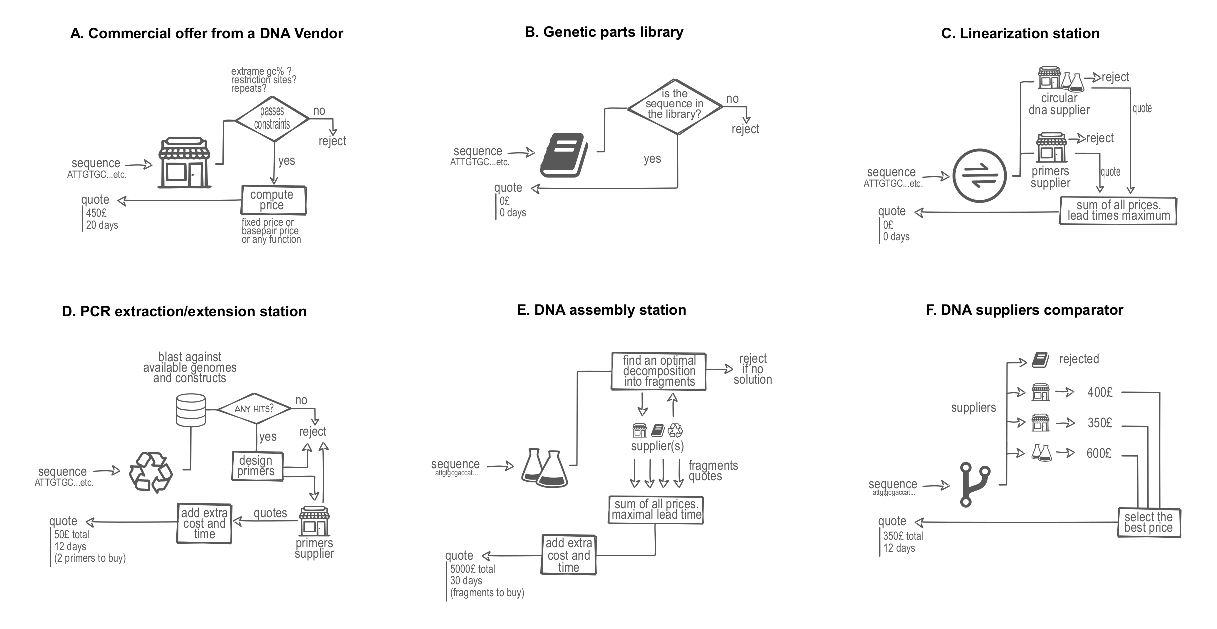
\includegraphics[width=\textwidth]{figures/figure_6_supply_network_elements.eps}
  \caption{Internal mechanisms of built-in DNA supplier classes}
  \label{dna suppliers_internals}
\end{figure}


\begin{figure}[!tpb]
  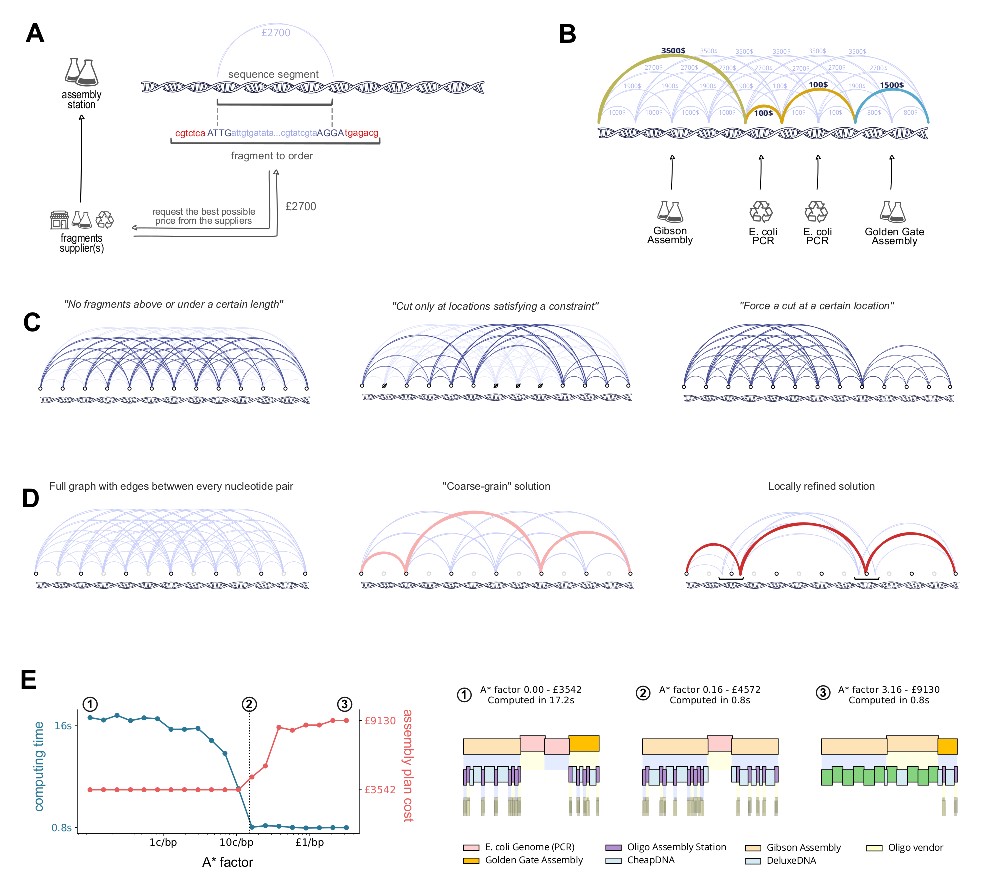
\includegraphics[width=\textwidth]{figures/figure_7_graph_algorithms.eps}
  \caption{Graph-based sequence decomposition methods.}
  \label{dna suppliers_internals}
\end{figure}

\begin{figure}[!tpb]
  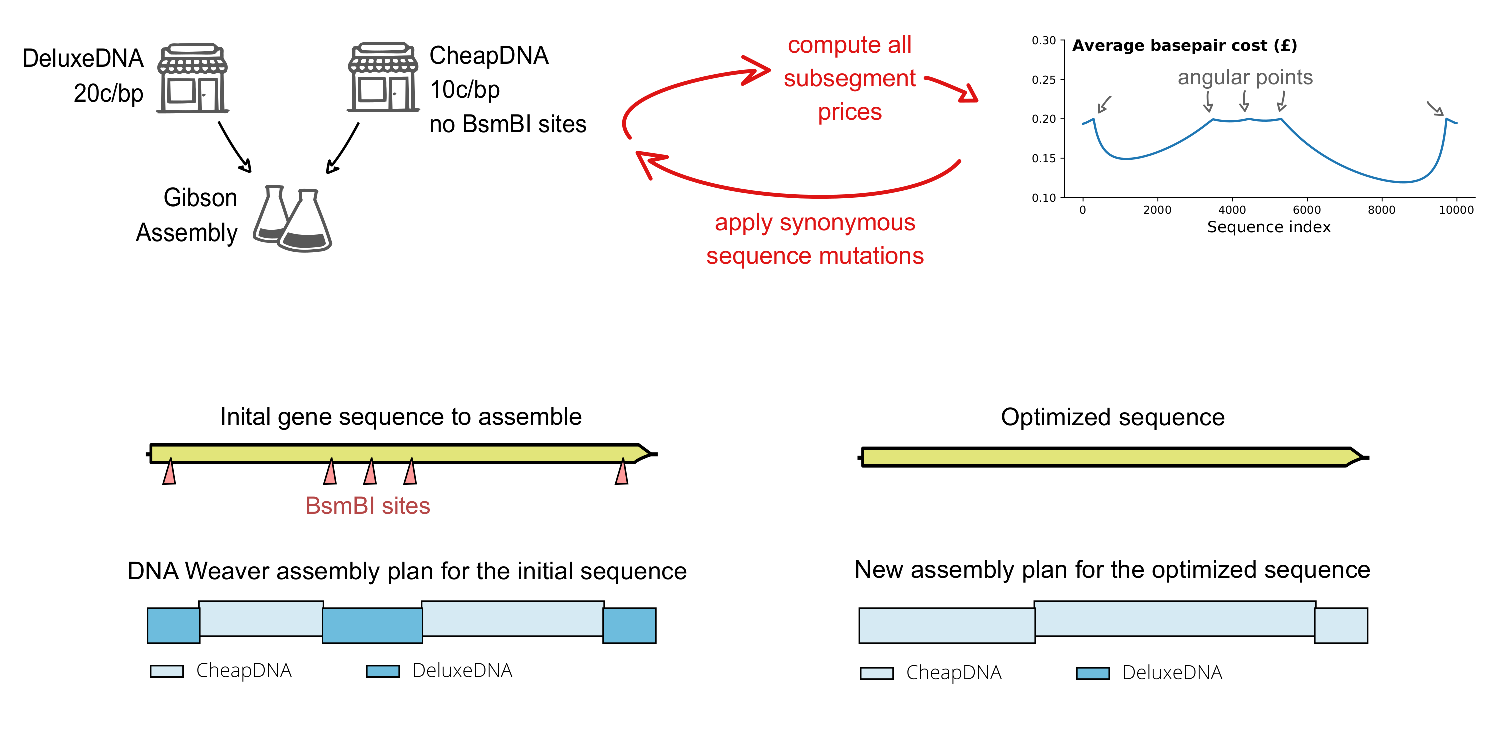
\includegraphics[width=\textwidth]{figures/figure_8_manufacturability-optimization.eps}
  \caption{Internal mechanisms of built-in DNA supplier classes}
  \label{dna suppliers_internals}
\end{figure}